\chapter{Prerequisites}

\r{The following sections are a non-exhaustive refresher on some of the important underlying concepts underpinning later concepts. Resources to further explore and learn these concepts are shared.}

\r{But first, let's start by answering the million dollar question: what is a tensor?  {Tensors}\index{tensor} are a generalization of matrices and can have an arbitrary number of dimensions (axis). The number of axes in a tensor is also called the {rank}\index{rank} of the tensor. For example, a $224\times224\times3$ image, would be considered a rank three tensor. If the batch dimension were included, ($n\times224\times224\times3$, where $n$ is the number of samples in a batch), we would have a rank four tensor.}


\section{Math Notation}

\r{Depending on the resource, the level of formal math education required to understand a se tion may vary greatly. In order to demystify some of the resources that do not expand on the proofs and notations, below are some of the symbols and XXXXX used in math notation and their interpretation in simple text/natural language form.}

\textcolor{green}{TODO: Show symbols and examples in both equation and simple text/natural language form.}

\textcolor{blue}{$\mathbb{R}$}

\section{Calculus}

% TODO: tie this to loss functions

\r{We won't be proving any theorems and we won't assign 45 questions due tomorrow. But, there is some basic terminology that should be revisited.}

\r{{Critical points}\index{critical points} or {stationary points}\index{stationary points} are points where the derivative is equal to zero and therefore doesn't provide any useful information about the gradient/slope (which direction and how far to move)}

\begin{figure}
	\centering
	\includegraphics[width=0.5\textwidth]{example-image-a}\hfil
	\caption{Graph of an example function and its derivative, \textcolor{green}{TODO}}
	\label{fig:calc_fn_deriv}
\end{figure}
\textcolor{green}{TODO: graph of function and it's derivative overlaid.}

\textcolor{blue}{There exist three main types of critical points:}

\begin{itemize}
	\item \textcolor{blue}{local minimum} -- 
	\item \textcolor{blue}{local maximum} -- 
	\item \textcolor{blue}{saddle point} -- 
\end{itemize}


% global + local min (strong and weak), inflection point
\begin{figure}[htp]
	\centering
	\includegraphics[width=0.3\textwidth]{example-image-a}\hfil
	\includegraphics[width=0.3\textwidth]{example-image-b}\hfil
	\includegraphics[width=0.3\textwidth]{example-image-c}
\caption{Types of critical points -- points with zero slope. From left to right, \textcolor{green}{TODO}}
\label{fig:calc_critical_points}
\end{figure}



\r{Local minimal are minimal values within a local region. It is possible, nearly certain actually, that a loss function for a given model will have many local minima. The point at which the absolute lowest value is present is considered the {global minimum}\index{global minimum}. Similarly, a value located at the absolute largest point is considered the {global maximum}\index{global maximum}. }

\begin{figure}
	\centering
	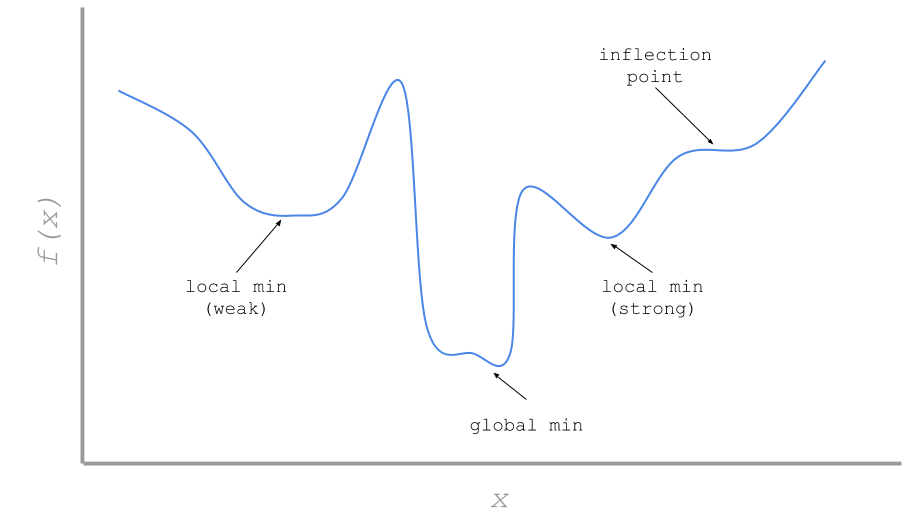
\includegraphics[width=0.8\textwidth]{./misc/critical_points.png}\hfil
	\caption{Example function with labeled local and global minima.}
	\label{fig:calc_fn_deriv}
\end{figure}

\subsection{Derivatives}

\r{The derivative of a fuction is the rate at which the value of the function changes with respect to how the a single input changes. The derivative can be thought of as the ratio between the functions output and input. A gradient is a generalization of a derivative to multi-input (multivariate) function.}

\TD{a partial derivative --- derivative with respect to one variable while all others are held constant.}


\r{Hyperplane: A subspace that consists of one dimension less than the dimensionality of the space it occupies e.g. a line in a 2D plot, or a 2D plane in a 3D environment}

\r{numerical differentiation is a process used to estimate derivatives numerically.}

\r{Two main methods for differentiating $f$ using a computational graph --- forward or reverse accumulation.}

\r{reverse accumulation\cite{linnainmaa1970representation} only requires a run to compute the complete gradient, but requires two passes through the graph (forward and reverse). \TD{more}}

\TD{importance of reverse accumulation in backpropagation\cite{rumelhart1988learning}}

\r{calculated by calculating the change over an infinitesimally small step \TD{illustration?}.}

\r{in theory, the smaller the step, the accurate the derivative estimate, however, in practice, steps that become too small may result in numerical errors}

\r{a place where the derivative is zero may also be called a stationary point}

\r{The step may be definited by the forward difference, the central diference, or the backward difference. \TD{figure?}}

% TODO: there likely is a better source for this.
\r{default step size is are the square (or cube) root of the machine precison for pointing point values\cite{kochenderfer2019algorithms} and are used as a balance between round-off error and step size error }

\r{more information on derivatives\cite{griewank2008evaluating}}

\subsection{Chain Rule}

\r{(not the chain rule of probability)}



\section{Boolean Logic}

\TD{TODO: background/overview on boolean logic and importance}

\TD{TODO: Examples}


\section{Linear Algebra}

\subsection{Overview}

\textcolor{green}{TODO: background/overview on linear algebra and importance}

\textcolor{green}{TODO: Examples}

\subsubsection{Scalars (0D tensors)}

\textcolor{green}{TODO: diagram}

\textcolor{blue}{scalar -- single value (not a vector or matrix)}

\textcolor{green}{example: a single value}


\subsubsection{Vectors (1D tensors)}

\textcolor{green}{TODO: diagram}

\textcolor{blue}{vectors -- denoted by lowercase names}

\textcolor{blue}{vector: an $n x 1$ matrix. A $12 x 1$ vector may be considered a 12 dimension vector.}

\textcolor{blue}{1-indexed or 0-indexed. In this document, we will only use 0-indexed terms}

\textcolor{green}{example: a ``list'' of features}


\subsubsection{Matrices (2D tensors)}

\textcolor{green}{TODO: diagram}

\textcolor{blue}{Matrix -- written as (rows x columns)}

\textcolor{blue}{$M_{i,j}$ means matrix entry at ($i$,$j$), or $i$th row, $j$th column}


\textcolor{blue}{Matrices -- denoted by uppercase names}

\textcolor{green}{example: a grayscale (single color channel image)}



\subsection{Matrix Arithmetic}

\textcolor{blue}{{element-wise}\index{element-wise} operations: operations that are applied independently to each entry. These types of operations lend themselves nicely to parallelization/vectorization}

\textcolor{blue}{dot product --- \textcolor{green}{TODO: visualization of dot product inputs and output}}

\subsubsection{Matrices}

\paragraph{Addition, Subtraction}

\paragraph{Multiplication, Division}

\subsubsection{Scalar}

\paragraph{Addition, Subtraction}

\paragraph{Multiplication, Division}



\section{Graph Theory}

\textcolor{green}{TODO: Examples}

\textcolor{blue}{computational graph}

\textcolor{blue}{operation}

